\documentclass[12pt]{article}
\usepackage[T1]{fontenc}
\usepackage[utf8]{inputenc}
\usepackage{url}
\usepackage{enumerate}
\usepackage[top=3cm, bottom=3cm]{geometry}
\usepackage{graphicx} 
\usepackage{natbib}
\usepackage{listings}
\usepackage{float}
\usepackage{amsmath}
\usepackage{amsfonts}
\usepackage{amssymb}
\usepackage{color}
\usepackage[parfill]{parskip}
\bibpunct{[}{]}{,}{a}{}{;}
\setcitestyle{super}

% Variables
\newcommand{\assignmentname}{Flow networks}

\begin{document}

\title{\assignmentname}

\maketitle
\thispagestyle{empty}

\subsubsection*{Flow network}

A \underline{flow network} consists of a digraph $G = (V, E)$ with a nonnegative capacity $c(u,v), \forall (u,v) \in E$, and a source $s \in V$, sink $ t\in V, s \neq t$.
We don't allow anti-parallel edges or self loops:

\begin{figure}[h]
  \centering
    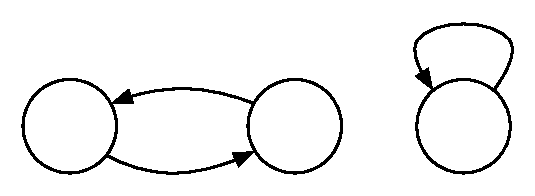
\includegraphics[width=0.3\textwidth]{figures/1}
\end{figure}

\subsubsection*{Constraints}

A flow in $(G, s, t, c)$ is a function $f: VxV \rightarrow \mathbb{R}$ such that:

\begin{enumerate}
  \item $\forall (u,v) \in V, 0 \geq f(u,v) \leq c(u,v)$ - \textbf{capacity constraint}
  \item $\forall u \in V \setminus \{s, t\}, \sum_{v\in V} f(u,v) = \sum_{v \in V} f(v,u)$ - \textbf{flow conservation}
\end{enumerate}

\subsubsection*{Flow value}

The value $|f|$ of $f$ is defined as $$|f| = \sum_{v \in V} f(s,v) - \sum_{v \in V} f(v, s)$$

\subsubsection*{The max flow problem}

Finding $f$ that maximizes the flow value $|f|$.

\subsubsection*{Residual capacity}

Given flow $f$ in $G$, define for any $(u,v) \in VxV$, \underline{residual capacity} of $(u,v)$ to be

\begin{align*}
  c_f(u,v) = \begin{cases}
               c(u,v) - f(u,v) & \text{if } (u,v) \in E\\
               f(v,u)          & \text{if } (v,u) \in E\\
               0               & \text{otherwise}
           \end{cases}
\end{align*}

\begin{figure}[h!]
  \centering
    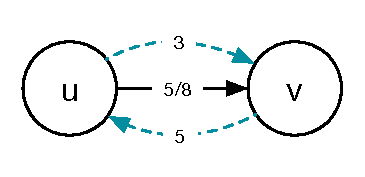
\includegraphics[width=0.4\textwidth]{figures/2}
\end{figure}

\subsubsection*{Residual network and augmented flow}

\underline{Residual network} $G_f$ is the flow network $(v, E_f)$, $E_f = \{ (u,v) \in VxV : c_f(u,v) > 0\}$.

Given flow $f$ in $G$ and a flow $f'$ in $G_f$, we define \underline{augmented flow} $f \uparrow f'$ as:

\begin{align*}
  (f \uparrow f')(u,v) = \begin{cases}
                          f(u,v) + f'(u,v) - f'(v,u) & \text{if } (u,v) \in E\\
                          0                          & \text{otherwise}
                         \end{cases}
\end{align*}

\subsubsection*{Ford-Fulkerson method}

Start with $f = 0$.\\
while there exists a path from $s$ to $t$ in $G_f$:\\
send as much flow as possible along $p$ to get $f'$ in $G_f$ and update $f \leftarrow f \uparrow f'$

\subsubsection*{\color{blue}Lemma} 

Given flow $f$ in $G$, flow $f'$ in $G_f$, then $f \uparrow f'$ is a flow in $G$ with value $|f \uparrow f'| = |f| + |f'|$.

\subsubsection*{\color{red}Proof}

 \begin{figure}[h!]
  \centering
    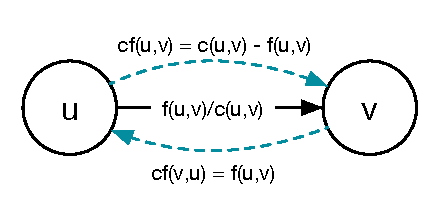
\includegraphics[width=0.5\textwidth]{figures/3}
\end{figure}

\underline{Verify using capacity constraint}

Observe that $c_f(v,u) = f(u,v)$ according to the residual capacity explanation here above. Therefore, the flow $f'(v,u) \leq c_f(v,u) = f(u,v)$ and:

\begin{align*}
  (|f \uparrow f'|)(u,v) &=    f(u,v) + f'(u,v) - f'(v,u) & \text{by definition here above}\\
                         &\geq f(u,v) + f'(u,v) - f(u,v)  & \text{because } f'(u,v) \leq f(u,v)\\
                         &=    f'(u,v) \\
                         &\geq 0
\end{align*}

and:

\begin{align*}
  (|f \uparrow f'|)(u,v) &=    f(u,v) + f'(u,v) - f'(v,u) & \text{by definition here above}\\
                         &\leq f(u,v) + f'(u,v)           & \text{because flows are nonnegative}\\
                         &\leq f(u,v) + c_f(u,v)          & \text{capacity constraints}\\
                         &=    f(u,v) + c(u,v) - f(u,v)   & \text{by definition of } c_f\\
                         &=    c(u,v).
\end{align*}

\underline{Verify using flow conservation}

For $u \in V \setminus \{s,t\}$,
\begin{align*}
  \sum_{v \in E}(f \uparrow f')(u,v) &= \sum_{v \in V}(f(u,v) + f'(u,v) - f'(v,u)) \\
                                     &= \sum_{v \in V}f(u,v) + \sum_{v \in V}f'(u,v) - \sum_{v \in V}f'(v,u) \\
                                     &= \sum_{v \in V}f(v,u) + \sum_{v \in V}f'(v,u) - \sum_{v \in V}f'(u,v) \\
                                     &= \sum_{v \in V}(f(v,u) + f'(v,u) - f'(u,v)) \\
                                     &= \sum_{v \in V}(f \uparrow f')(v,u)
\end{align*}


\subsubsection*{Cuts}

\begin{figure}[h!]
  \centering
    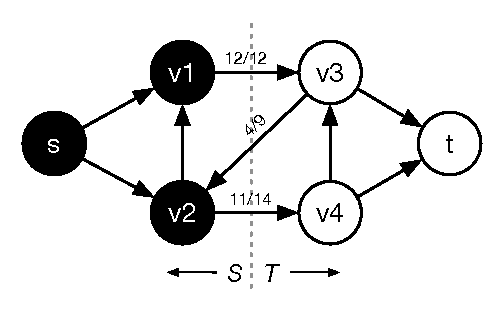
\includegraphics[width=0.5\textwidth]{figures/5}
\end{figure}

A cut is a partition of $V$ into two subsets $(S,T)$ such that $s \in S$ and $t \in T$.

\subsubsection*{Capacity of cut}

The capacity of $(S,T)$ is:

  $$ c(S,T) = \sum_{u \in S}\sum_{v \in T} c(u,v) $$

The capacity of the cut here above is $12 + 14 = 26$.

\subsubsection*{Net flow of cut}

Given flow $f$ in G, the flow across $(S,T)$ is:

  $$ f(S,T) = \sum_{u \in S}\sum_{v \in T} f(u, v) -  \sum_{u \in S}\sum_{v \in T} f(v, u)$$

The net flow of the cut in the graph here above is $12 + 11 - 4 = 19$.

\subsubsection*{\color{blue}Lemma}

For any cut $(S, T)$, $f(S,T) = |f|$.

\subsubsection*{\color{red}Proof}

\dots

\subsubsection*{\color{blue}Corollary}

Given any flow $f$ in $G$ and any cut $(S, T)$, $|f| \leq c(S, T)$. 

\subsubsection*{\color{red}Proof}

\begin{align*}
  |f| &=    f(S,T) \\
      &=    \sum_{u \in S}\sum_{v \in T} f(u, v) -  \sum_{u \in S}\sum_{v \in T} f(v, u)\\
      &\leq \sum_{u \in S}\sum_{v \in T} f(u, v)\\
      &\leq \sum_{u \in S}\sum_{v \in T} c(u, v)\\
      &=c(S,T)
\end{align*}

\subsubsection*{Max-flow min-cut theorem}

Given flow $f$ in $G$, the following three statements are equivalent:

\begin{enumerate}
  \item $f$ is a max flow
  \item there is no augmenting path in $G_f$
  \item there is a cut $(S,T)$ such that $|f| = c(S, T)$.
\end{enumerate}

\subsubsection*{\color{red}Proof}

\underline{(1) => (2)}

Assume there is a path $p$ from $s$ to $t$ in $G_f$. Augmenting $f$ with $f_p$ gives flow $f \uparrow f_p$ in $G$ and its value is $$|f \uparrow f_p| > |f|$$ which contradicts the assumption that $f$ is a maximum flow.

\underline{(2) => (3)}

We assume that $G_f$ has no augmenting path, meaning that there is no path between $s$ and $t$ in $G_f$. Let's define $S = \{v \in V : \text{there exists a path from } s \text{ to } v \text{ in } G_f\}$ and $T = V \setminus S$. $(S,T)$ is therefore a cut. We now consider a pair of vertices $u \in S$ and $v \in T$. If $(u,v) \in E$, we must have that $f(u,v) = c(u,v)$ because otherwise we would have $(u,v) \in G_f$ which would place $v$ in $S$ (\textit{if there exists an path from s to u, and u to v, then there is a path from s to v}). Similarly, if $(v,u) \in E$, we must have that $f(v,u) = 0$ because otherwise we would have $c_f(u,v) = f(v,u)$ and $(u,v) \in G_f$ which would place $v$ in $S$.

We thus have:

\begin{align*}
  f(S,T) &=  \sum_{u \in S}\sum_{v \in T} f(u, v) -  \sum_{u \in S}\sum_{v \in T} f(v, u)\\
         &=  \sum_{u \in S}\sum_{v \in T} c(u, v) -  \sum_{u \in S}\sum_{v \in T} 0\\
         &=  c(S,T)
\end{align*}

\begin{figure}[h!]
  \centering
    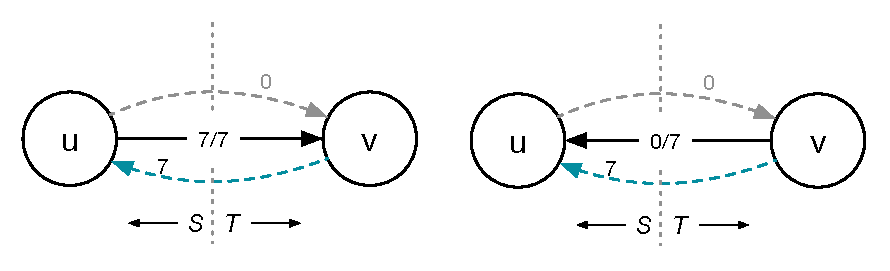
\includegraphics[width=1\textwidth]{figures/6}
\end{figure}

\underline{(3) => (1)}

By the corollary that $|f| \leq c(S,T)$ for all cuts $(S,T)$, the condition that $|f| = c(S,T)$ thus implies that $f$ is the maximum flow. 


\subsubsection*{Edmonds-Karp}

Implementation of Ford-Fulkerson where augmenting paths are shortest paths in $G_f$.

\subsubsection*{\color{blue}Lemma}

Consider any $v \in V \setminus \{s, t\}$. Then $\delta_f(s,v)$ is monotonically non-decreasing when running Edmond-Karp.

\subsubsection*{\color{red}Proof}

\textit{$\delta_f(s,u)$ is the shortest path distance from s to u in $G_f$}

Assume otherwise and let $f$ be the first flow where distance to some $v \in V \setminus \{s,t\}$ goes down when augmenting flow. Let $f'$ be the next flow $\delta_{f'}(s,v) < \delta_f(s,v)$. Pick $v$ such that $\delta_{f'}(S,v)$ is minimized. Let $p$ be a shortest path in $G_f$ from $s$ to $v$:

$$p = s \sim u \rightarrow v$$.
$$\delta_{f'}(s,v) = \delta_{f'}(s,u) + 1$$

By choice of $v$, $\delta_{f'}(s,u) \geq \delta_f(s,u)$
\end{document}
% End of document.







